\documentclass[12pt]{article} 
\usepackage[left=2cm, right=2cm, top=1.5cm, bottom=1.5cm]{geometry} 
\usepackage[pages=some]{background}
\usepackage{subcaption}
\usepackage{graphicx}


\begin{document}




\pagebreak
\begin{figure}[h]
  \begin{center}
    \includegraphics*[width=0.89\linewidth]{img/exp_3a.png}
  \end{center}
\end{figure}



\begin{figure}[h]
    \centering
    \begin{subfigure}{0.3\textwidth}
        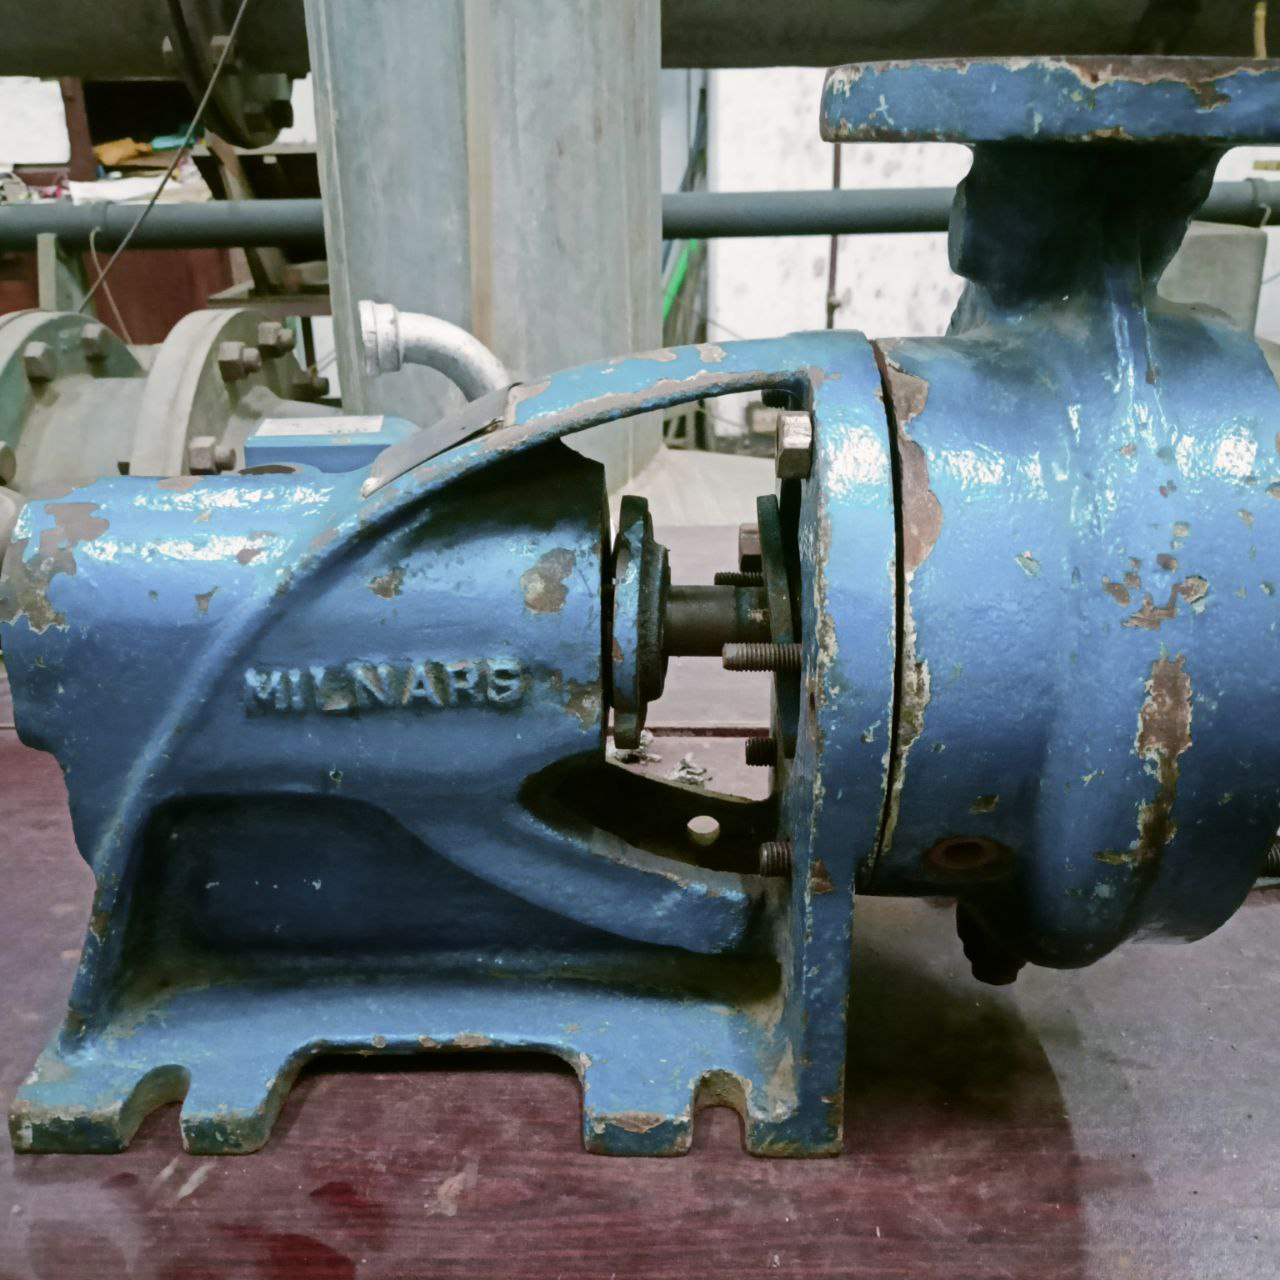
\includegraphics[width=\linewidth]{img/p_01.jpg}
        \caption{Pump}  
    \end{subfigure}
    \hfill
    \begin{subfigure}{0.3\textwidth}
        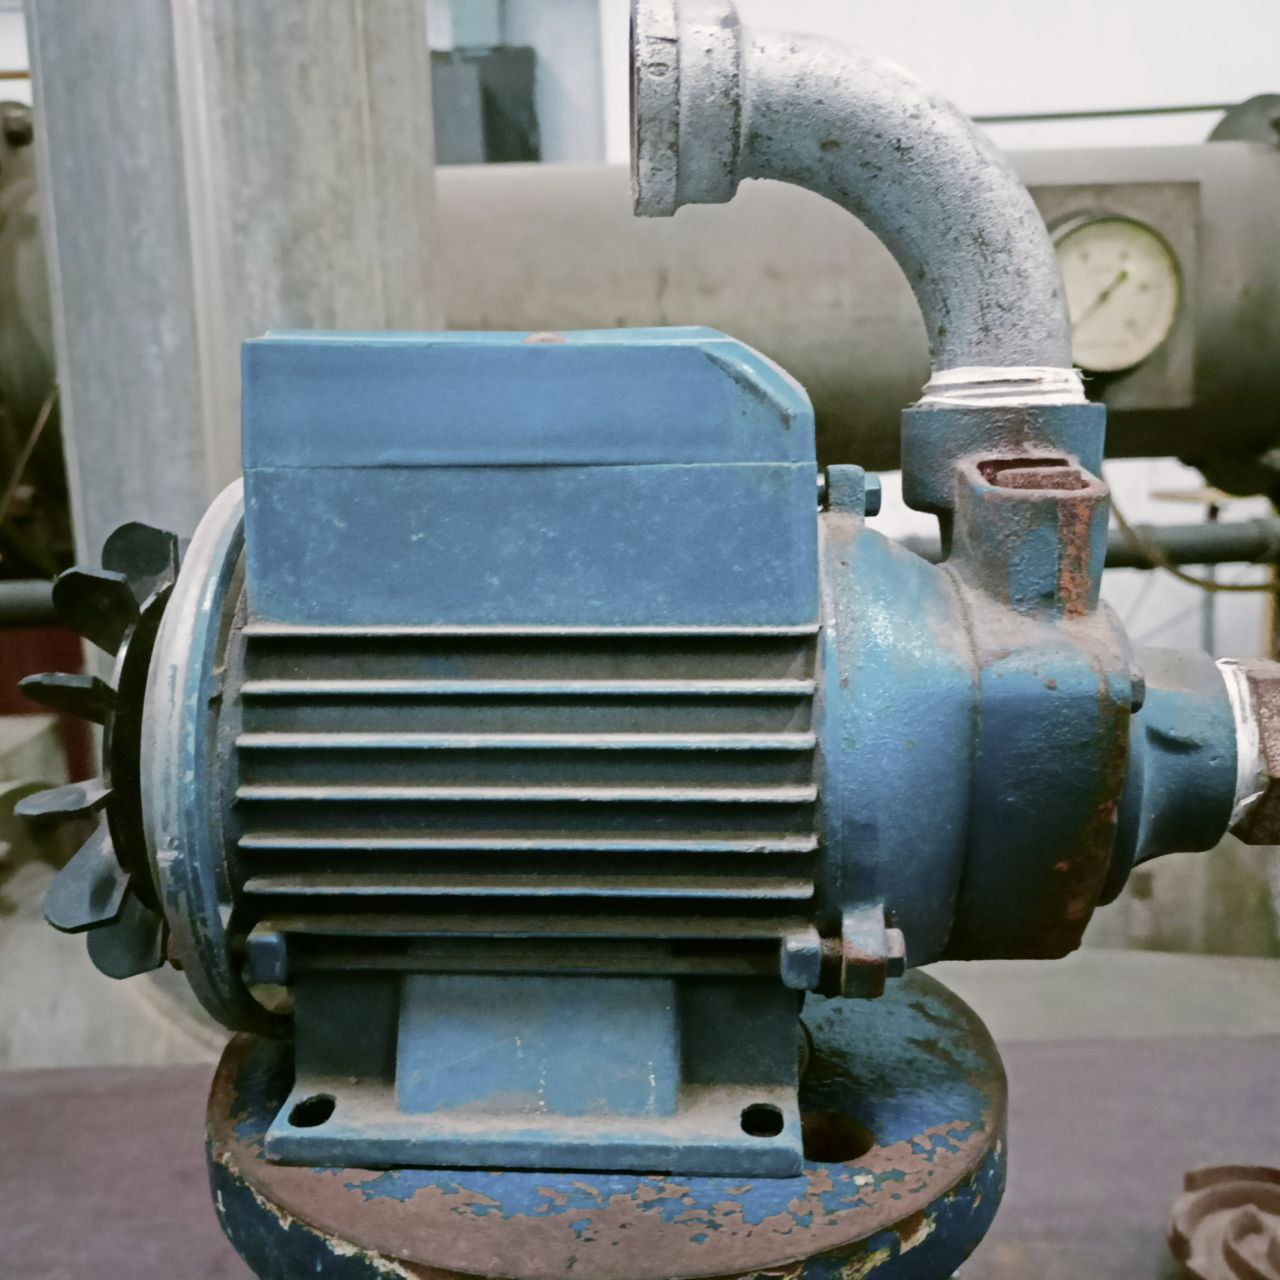
\includegraphics[width=\linewidth]{img/p_02.jpg}
        \caption{Motor}
    \end{subfigure}
    \hfill
    \begin{subfigure}{0.3\textwidth}
        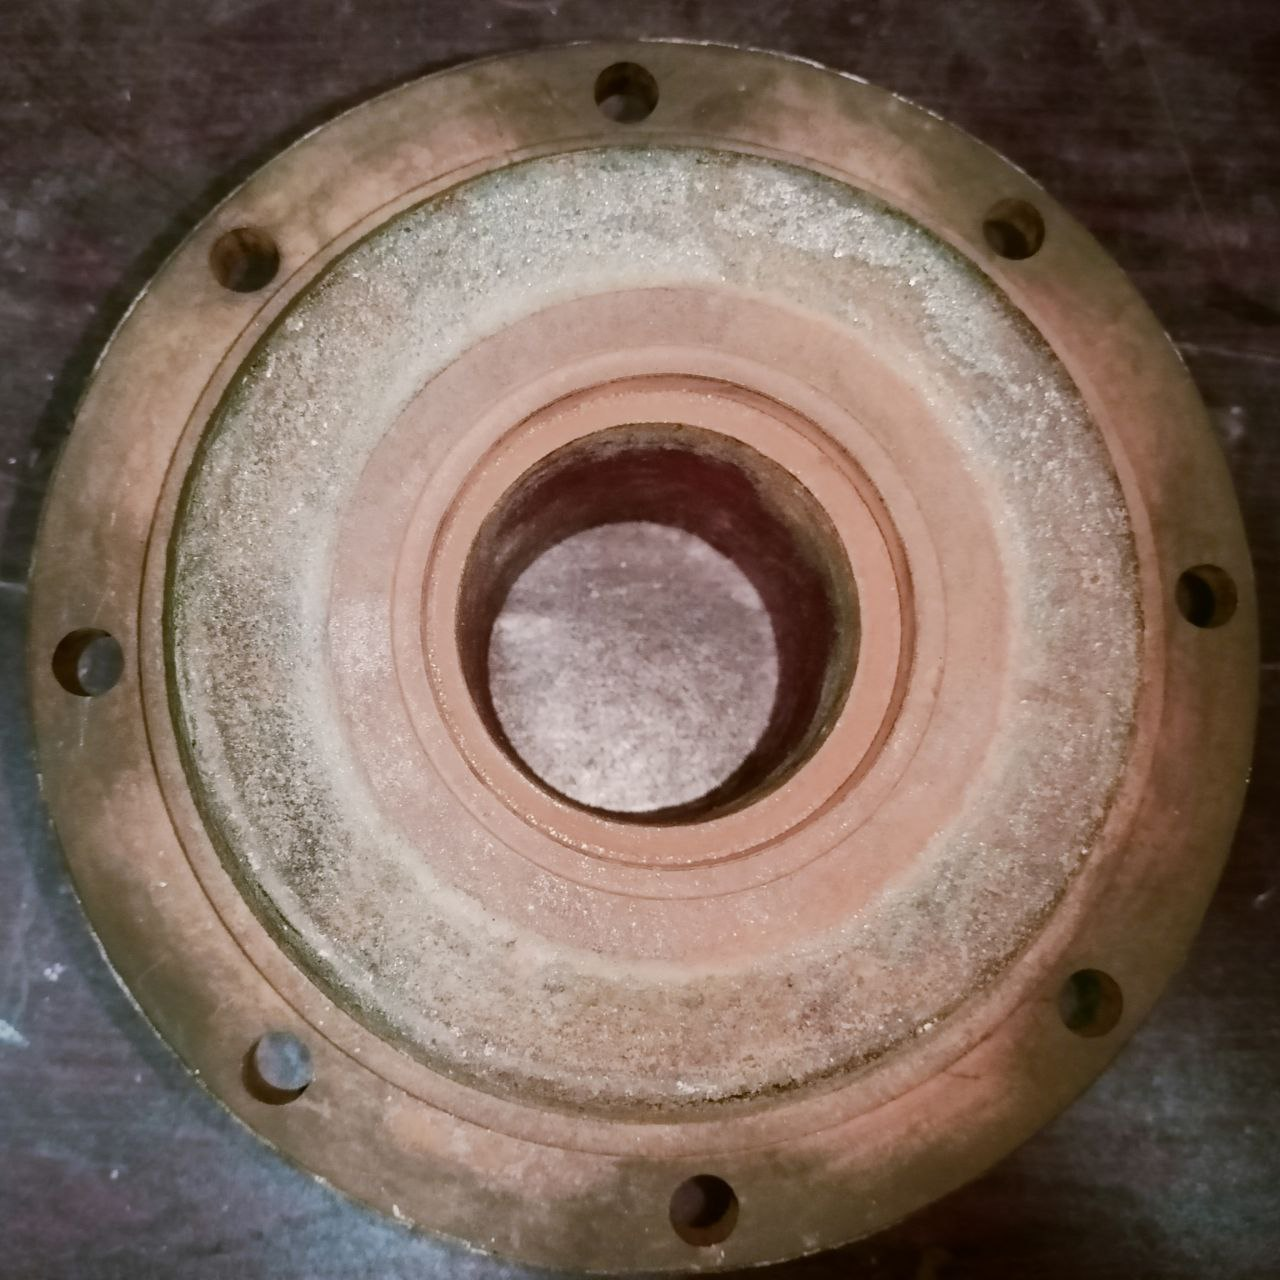
\includegraphics[width=\linewidth]{img/p_03.jpg}
        \caption{Image 3}
    \end{subfigure}
  
    \vspace{0.5cm}
  
    \begin{subfigure}{0.3\textwidth}
        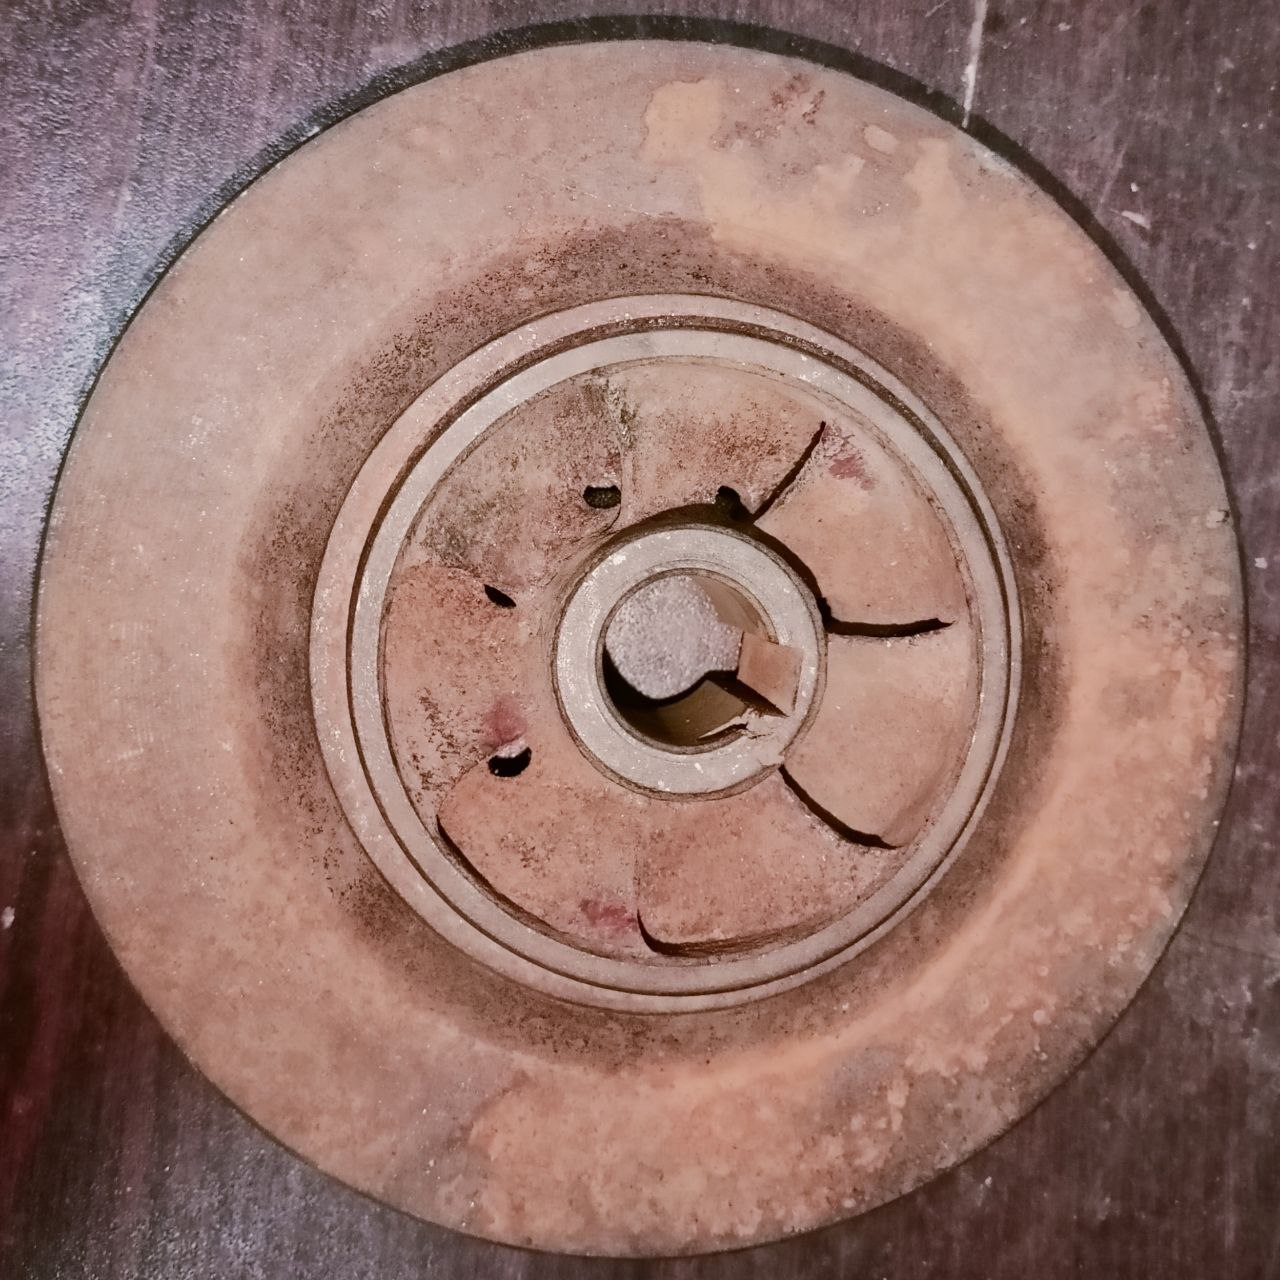
\includegraphics[width=\linewidth]{img/p_04.jpg}
        \caption{Image 4}
    \end{subfigure}
    \hfill
    \begin{subfigure}{0.3\textwidth}
        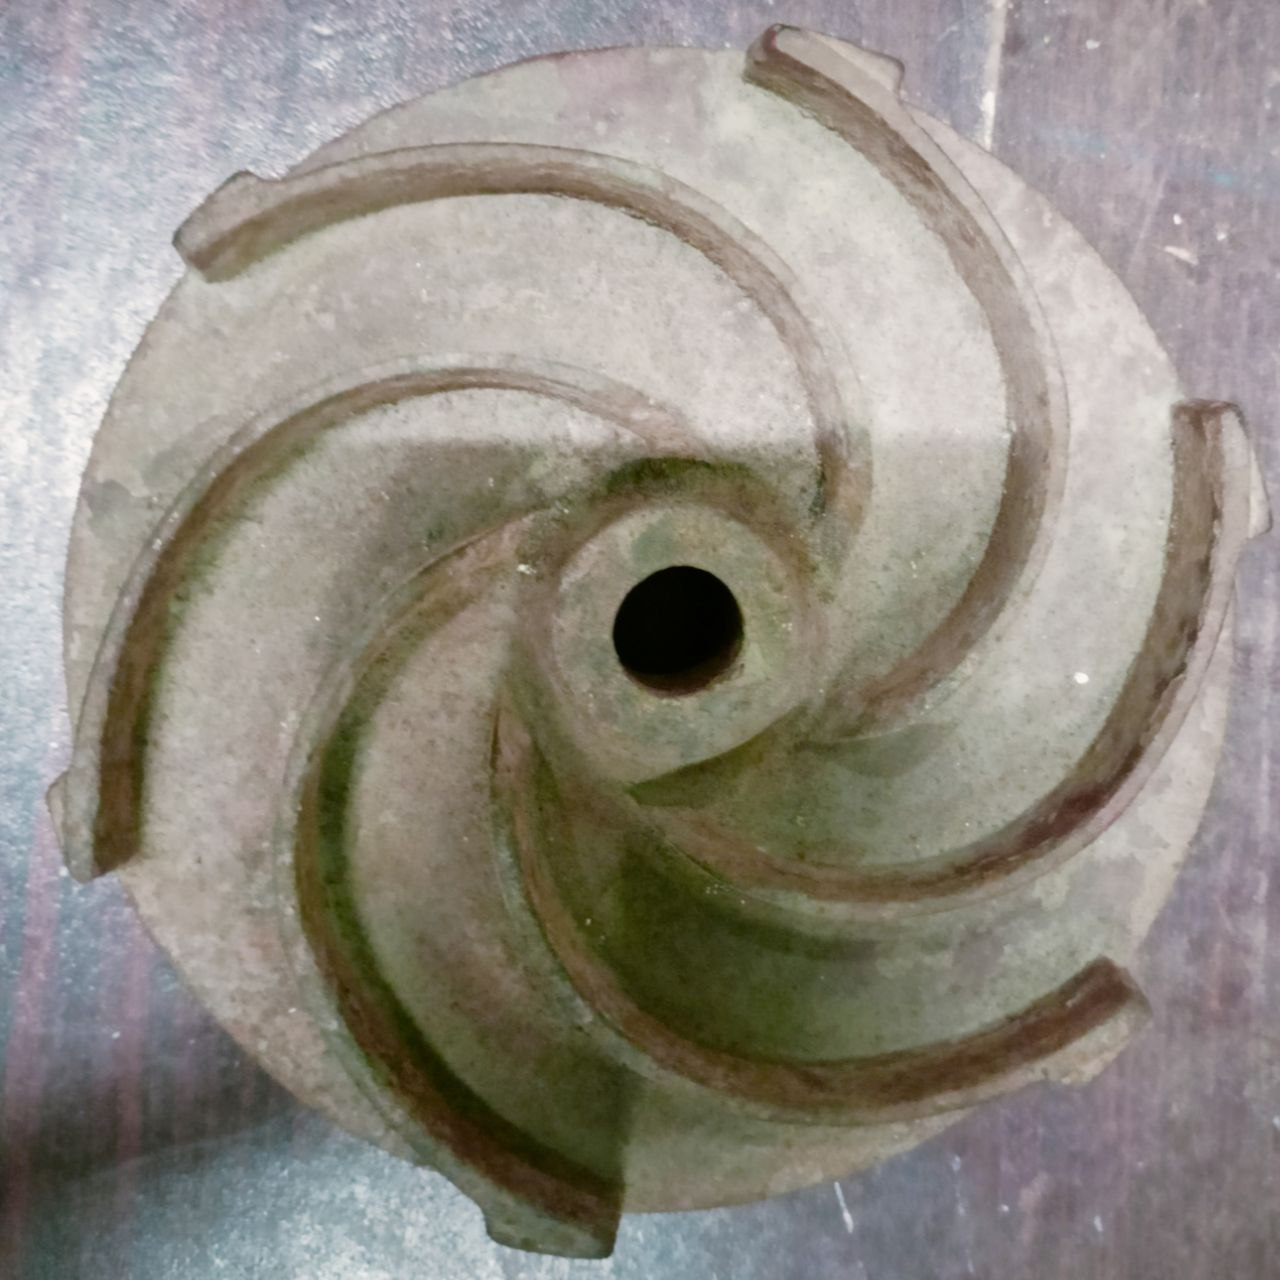
\includegraphics[width=\linewidth]{img/p_05.jpg}
        \caption{Image 5}
    \end{subfigure}
    \hfill
    \begin{subfigure}{0.3\textwidth}
        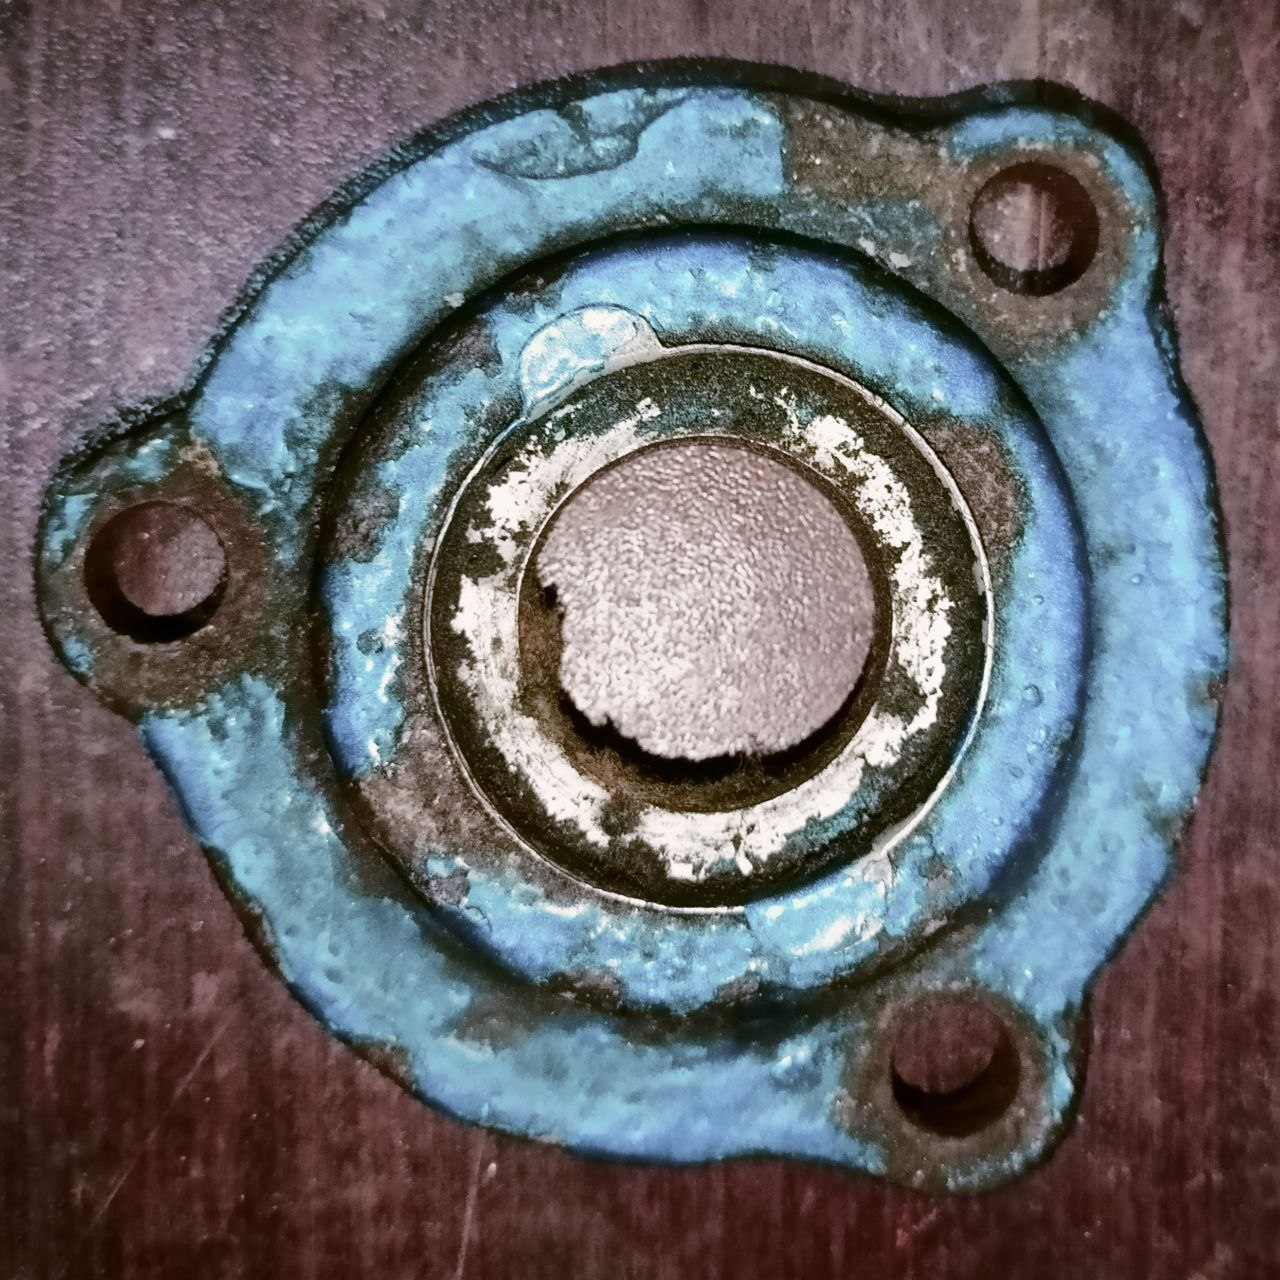
\includegraphics[width=\linewidth]{img/p_06.jpg}
        \caption{Image 6}
    \end{subfigure}
  
    \vspace{0.5cm}
  
    \begin{subfigure}{0.3\textwidth}
        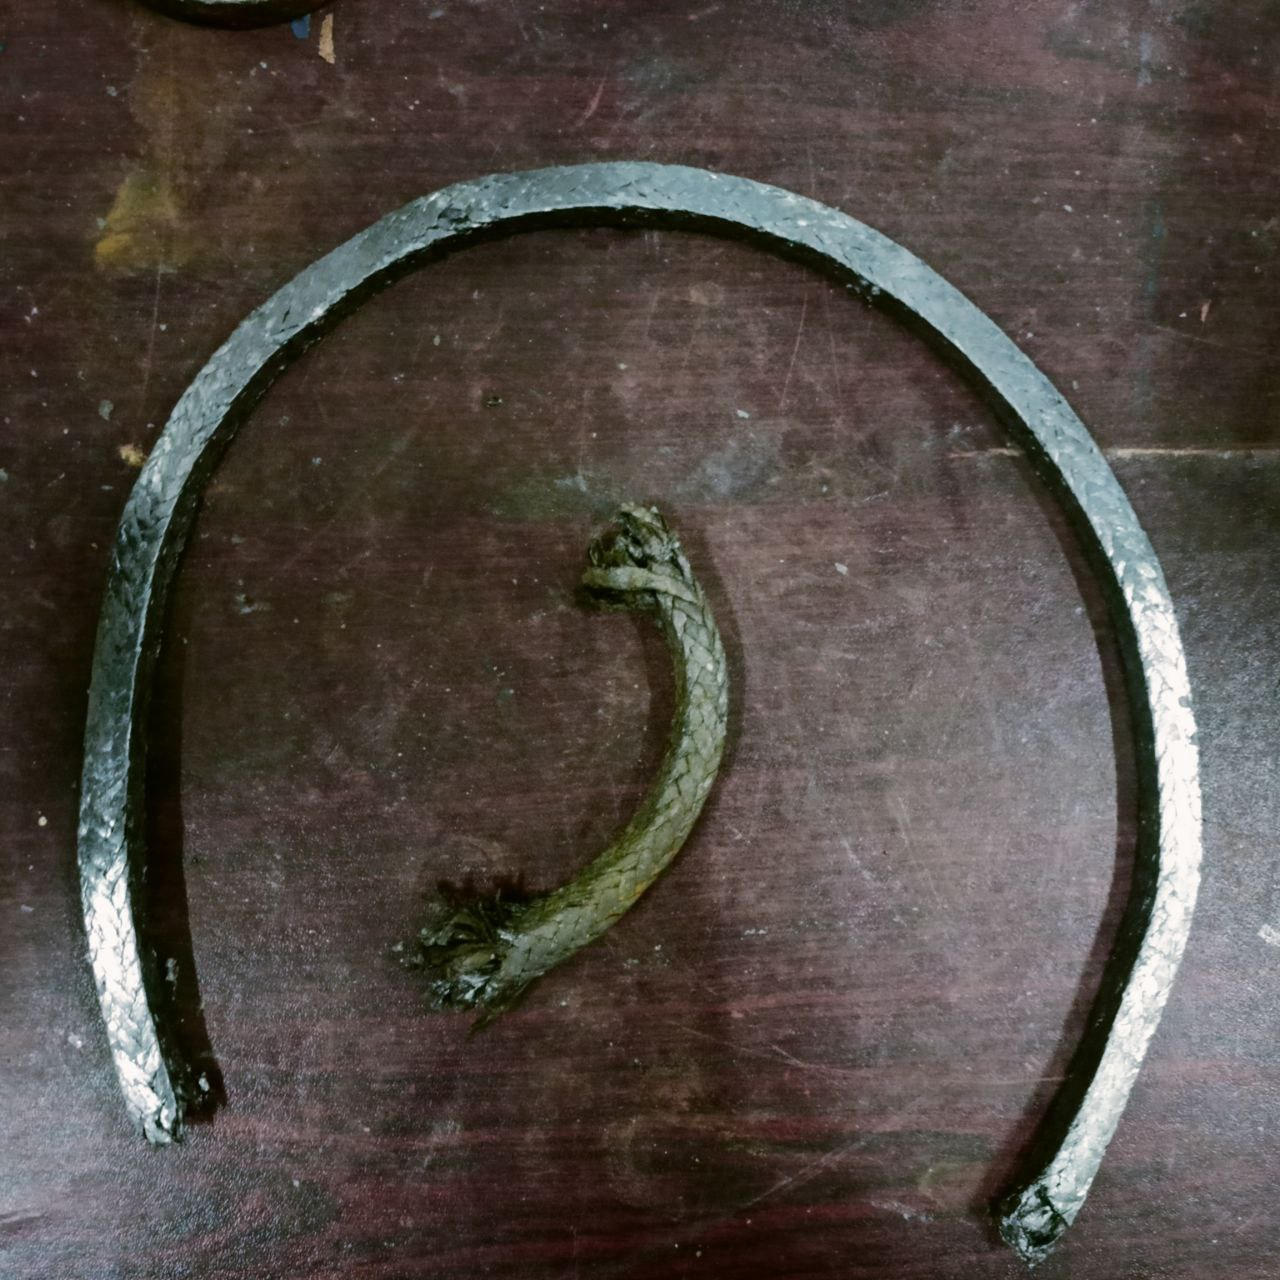
\includegraphics[width=\linewidth]{img/p_07.jpg}
        \caption{Image 7}
    \end{subfigure}
    \hfill
    \begin{subfigure}{0.3\textwidth}
        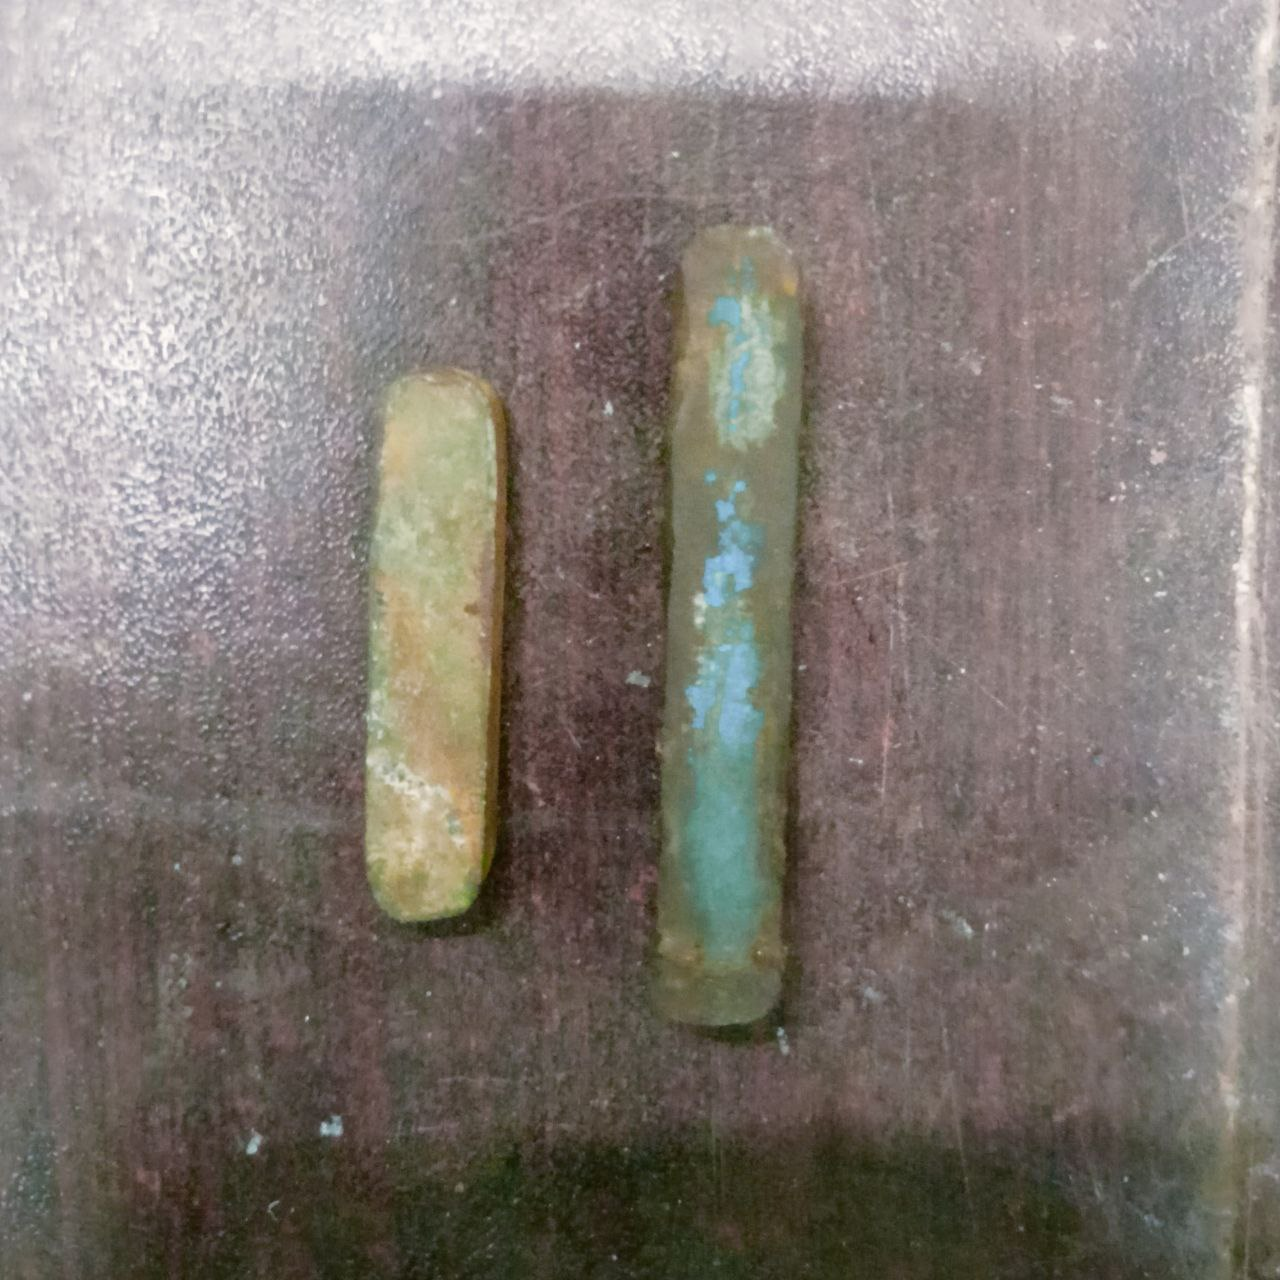
\includegraphics[width=\linewidth]{img/p_08.jpg}
        \caption{Image 8}
    \end{subfigure}
    \hfill
    \begin{subfigure}{0.3\textwidth}
        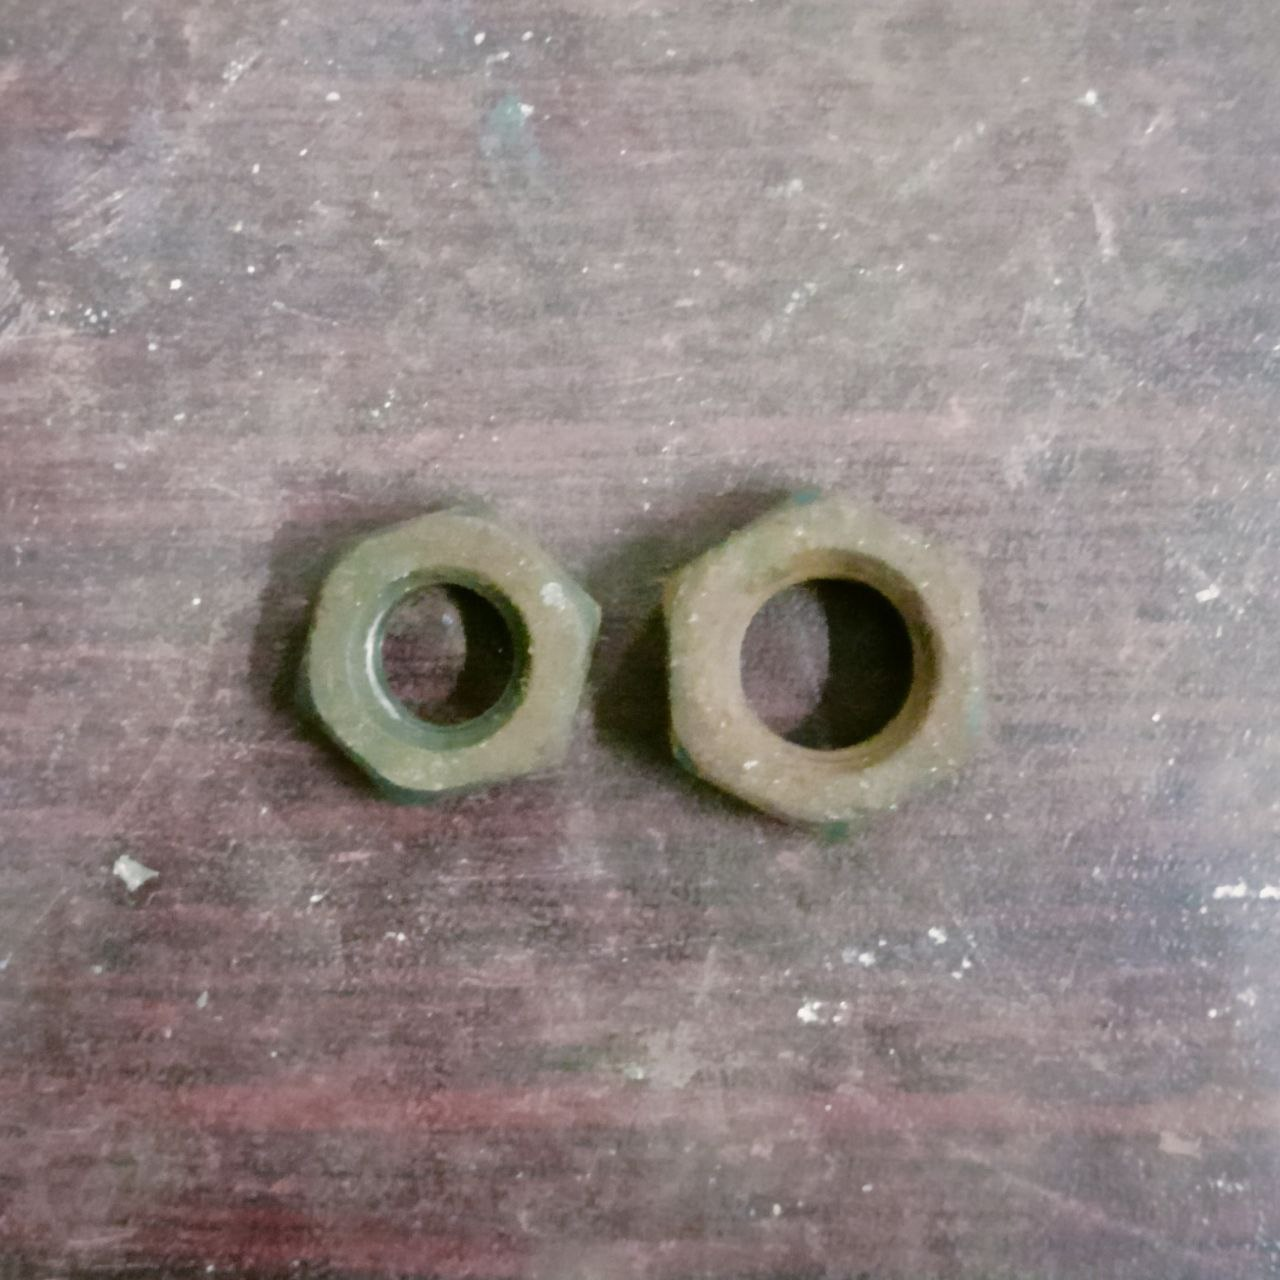
\includegraphics[width=\linewidth]{img/p_09.jpg}
        \caption{Image 9}
    \end{subfigure}
  
    \caption{Subplot Figure with 9 Images}
  \end{figure}

\end{document}